%!TEX root = main.tex

\toclesssection{Introduction and Motivation}

\begin{frame}{Introduction and Motivation}{The Simulation of Dynamic Systems}
  \begin{columns}
    \begin{column}[c]{0.6\textwidth}
      \uncover<1->{%
        \hi{\large Why do we need simulation?} \\
        It is used to \\
        \begin{itemize}\small
          \setlength{\itemsep}{0.0em}
          \item[\raisebox{-1pt}{\scalebox{0.8}{\faCogs}}] \emph{predict} the behavior
          \item[\raisebox{-1pt}{\scalebox{0.8}{\faConnectdevelop}}] \emph{design} and \emph{optimize}
          \item[\raisebox{-1pt}{\scalebox{0.8}{\faHourglassHalf}}] accelerate development and testing
          \item[\raisebox{-1pt}{\scalebox{0.8}{\faCarCrash}}] risk-free testing environment
          \item[\raisebox{-1pt}{\scalebox{0.8}{\faDollarSign}}] \emph{reduce} development costs
        \end{itemize}
      }
      \vspace{0.5em}
      \uncover<2->{%
        \hi{\large Simulations' \textbf{complexity} is increasing!} \\
        Higher \textbf{fidelity}, more \textbf{complexity}, more \dots \\
        \begin{itemize}\small
          \setlength{\itemsep}{0.0em}
          \item[\raisebox{-1pt}{\scalebox{0.8}{\faCog}}] components \\
          \item[\raisebox{-1pt}{\scalebox{0.8}{\faCompress}}] interactions \\
          \item[\raisebox{-1pt}{\scalebox{0.8}{\faDesktop}}] computational resources \\
          \item[\raisebox{-1pt}{\scalebox{0.8}{\faHourglassHalf}}] computation time
        \end{itemize}
      }
      \end{column}
    \begin{column}[c]{0.4\textwidth}
      \centering
      \visible<3->{\includegraphics[width=0.52\textwidth, trim={0cm 0cm 4.65cm 0cm}, clip]{figures/vehicle_modules.eps}}
    \end{column}
  \end{columns}
\end{frame}

\subsection{Dynamic Systems as a Collection of Subsystems}

\begin{frame}{Introduction and Motivation}{Dynamic Systems as a Collection of Subsystems}
  \begin{columns}
    \begin{column}[c]{0.6\textwidth}
      \begin{itemize}
        \item<1-> Complex systems are divided into \textbf{subsystems} \\
        \begin{small}
          \quad\, \begin{tabular}{ccc}
            \raisebox{-1pt}{\scalebox{0.8}{\textcolor{fg_sl_color}{\faCogs}}} mechanical &
            \raisebox{-1pt}{\scalebox{0.8}{\textcolor{fg_sl_color}{\faBolt}}} electrical &
            \raisebox{-1pt}{\scalebox{0.8}{\textcolor{fg_sl_color}{\faFire}}} thermal \\
            \raisebox{-1pt}{\scalebox{0.8}{\textcolor{fg_sl_color}{\faOilCan}}} hydraulic &
            \raisebox{-1pt}{\scalebox{0.8}{\textcolor{fg_sl_color}{\faWaveSquare}}} control & \dots
          \end{tabular}
        \end{small}
        \item<2-> Subsystems are modeled by \textbf{equations} \\
        \begin{small}
          \qquad \emph{algebraic} \\
          \qquad ordinary \emph{differential} \\
          \qquad \emph{differential-algebraic} \\
          \qquad other types
        \end{small}
        \item<3-> The \textbf{challenges} are \hic{\normalsize Speed \qquad Accuracy \qquad Efficiency}
      \end{itemize}
    \end{column}
    \begin{column}[c]{0.4\textwidth}
      \centering
      \only<1->{\includegraphics[width=\textwidth]{figures/vehicle_modules.eps}}
    \end{column}
  \end{columns}
\end{frame}

\subsection{Solution Approaches}

\begin{frame}{Introduction and Motivation}{Solution Approaches}
  \begin{columns}
    \begin{column}[c]{0.45\textwidth}
      The \textbf{solution} of these equations can be \dots \\
      \begin{itemize}[<+->]
        \item \textbf{Analytical} \\
        \begin{small}
          \qquad \textcolor{mycolor2!95!black}{deep understanding of the problem} \\
          \qquad \textcolor{mycolor2!95!black}{rare and difficult to achieve} \\
          \qquad \textcolor{mycolor5!95!black}{low computational resources}
        \end{small}
        \item \textbf{Numerical} \\
        \begin{small}
          \qquad \textcolor{mycolor5!95!black}{well-established and widely used} \\
          \qquad \textcolor{mycolor3!95!black}{parametricity loss} \\
          \qquad \textcolor{mycolor2!95!black}{high computational resources}
        \end{small}
        \item \textbf{Mixed analytical/numerical} \\
        \begin{small}
          \qquad \textcolor{mycolor3!95!black}{\emph{ad hoc}, for specific cases} \\
          \qquad \textcolor{mycolor5!95!black}{balance between the two approaches} \\
          \qquad \textcolor{mycolor5!95!black}{reduced computational resources}
        \end{small}
      \end{itemize}
    \end{column}
    \begin{column}[c]{0.6\textwidth}
      \centering
      \small
      \vspace{-2.0em}
      \begin{tabular}{>{\centering\arraybackslash} m{3.75cm} >{\centering\arraybackslash} m{3.75cm}}
        \visible<3->{\vspace{-3.0em}$\msmall{\begin{array}{c}
          \text{\hi{Tire-road interaction (A1-2)}} \\[0.25em]
          \mathbf{P} = \frac{1}{V} \int\nolimits_\mathcal{V} \text{proj}(\mathbf{x}, \partial\mathcal{G}) \, \text{d}\mathcal{\mathbf{x}} \\[0.1em]
          \mathbf{\hat{n}} = \int\nolimits_\mathcal{V} \mathbf{d}(\mathbf{x},\mathbf{h}_y) \, \text{d}\mathcal{\mathbf{x}}
        \end{array}}$ &
        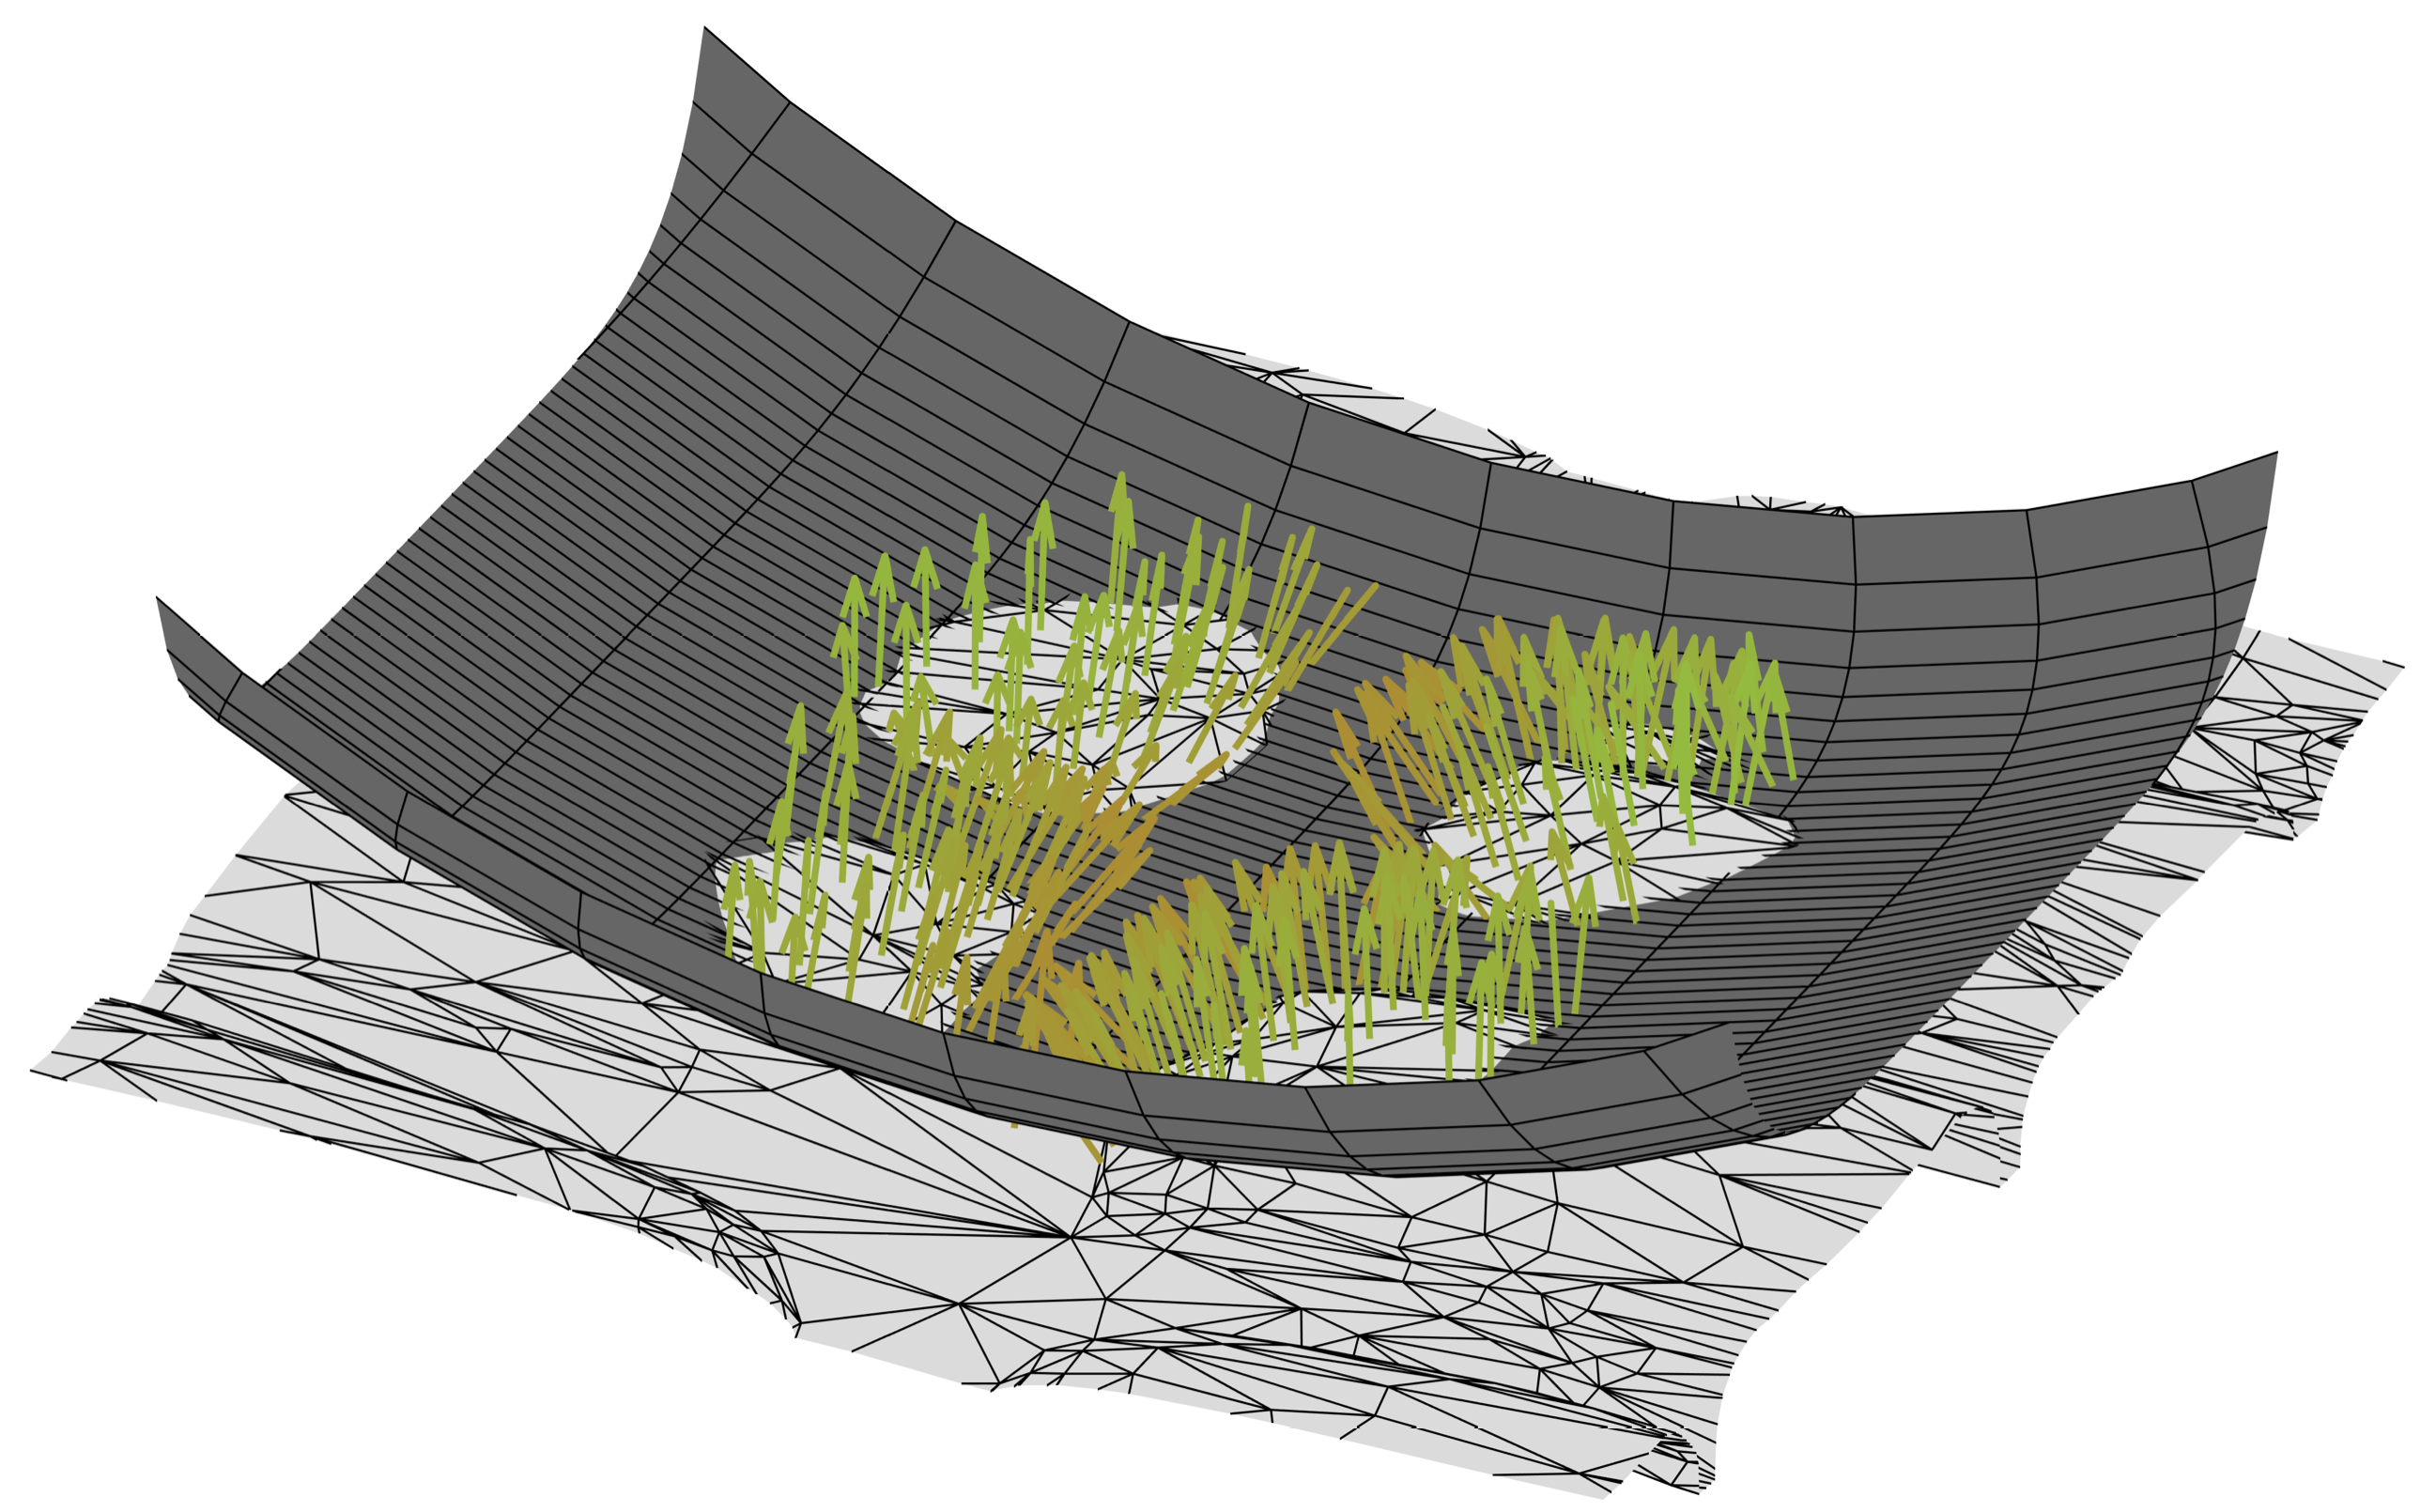
\includegraphics[width=0.4\textwidth]{figures/enve_intersection.png}} \\
        \visible<3->{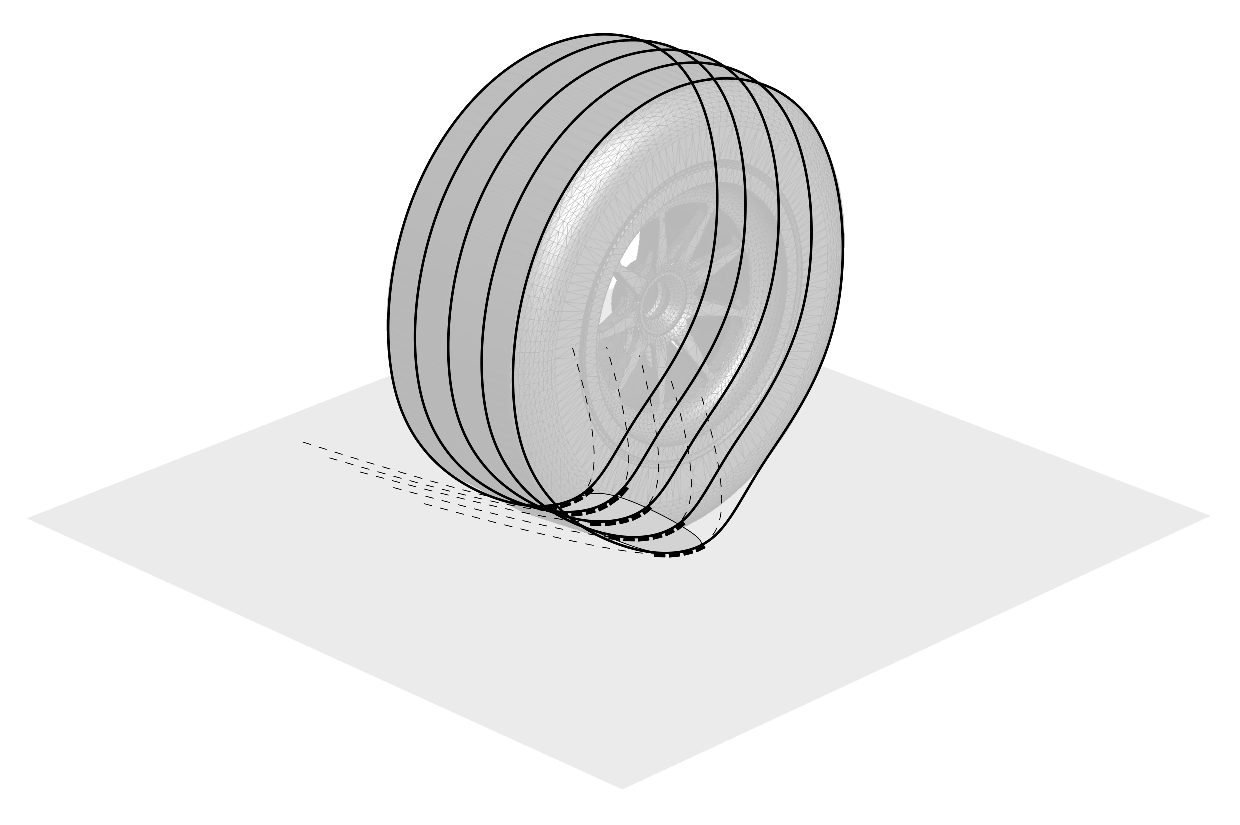
\includegraphics[
          width=0.35\textwidth, trim={4.5cm 3.5cm 4.5cm 0cm}, clip
          ]{figures/brush_model_simplified.eps} &
          \vspace{-3.0em}$\msmall{\begin{array}{c}
            \text{\hi{Tire model (A3)}} \\[0.25em]
            \mathbf{F}(F_z, \sigma_x, \sigma_y, \varphi, \gamma, p, T, t) \\[0.1em]
            \mathbf{M}(F_z, \sigma_x, \sigma_y, \varphi, \gamma, p, T, t)
          \end{array}}$} \\
          \visible<3->{\vspace{-2.0em}$\begin{array}{c}
            \text{\hi{Direct stiffness method (A4)}} \\[0.25em]
            \begin{bmatrix}
              \mathbf{K}_{ff} & \mathbf{K}_{fs} \\
              \mathbf{K}_{sf} & \mathbf{K}_{ss}
            \end{bmatrix} \begin{bmatrix}
              \mathbf{d}_{f} \\
              \mathbf{d}_{s}
            \end{bmatrix} = \begin{bmatrix}
              \mathbf{f}_{f} \\
              \mathbf{f}_{s}
            \end{bmatrix}
          \end{array}$ &
          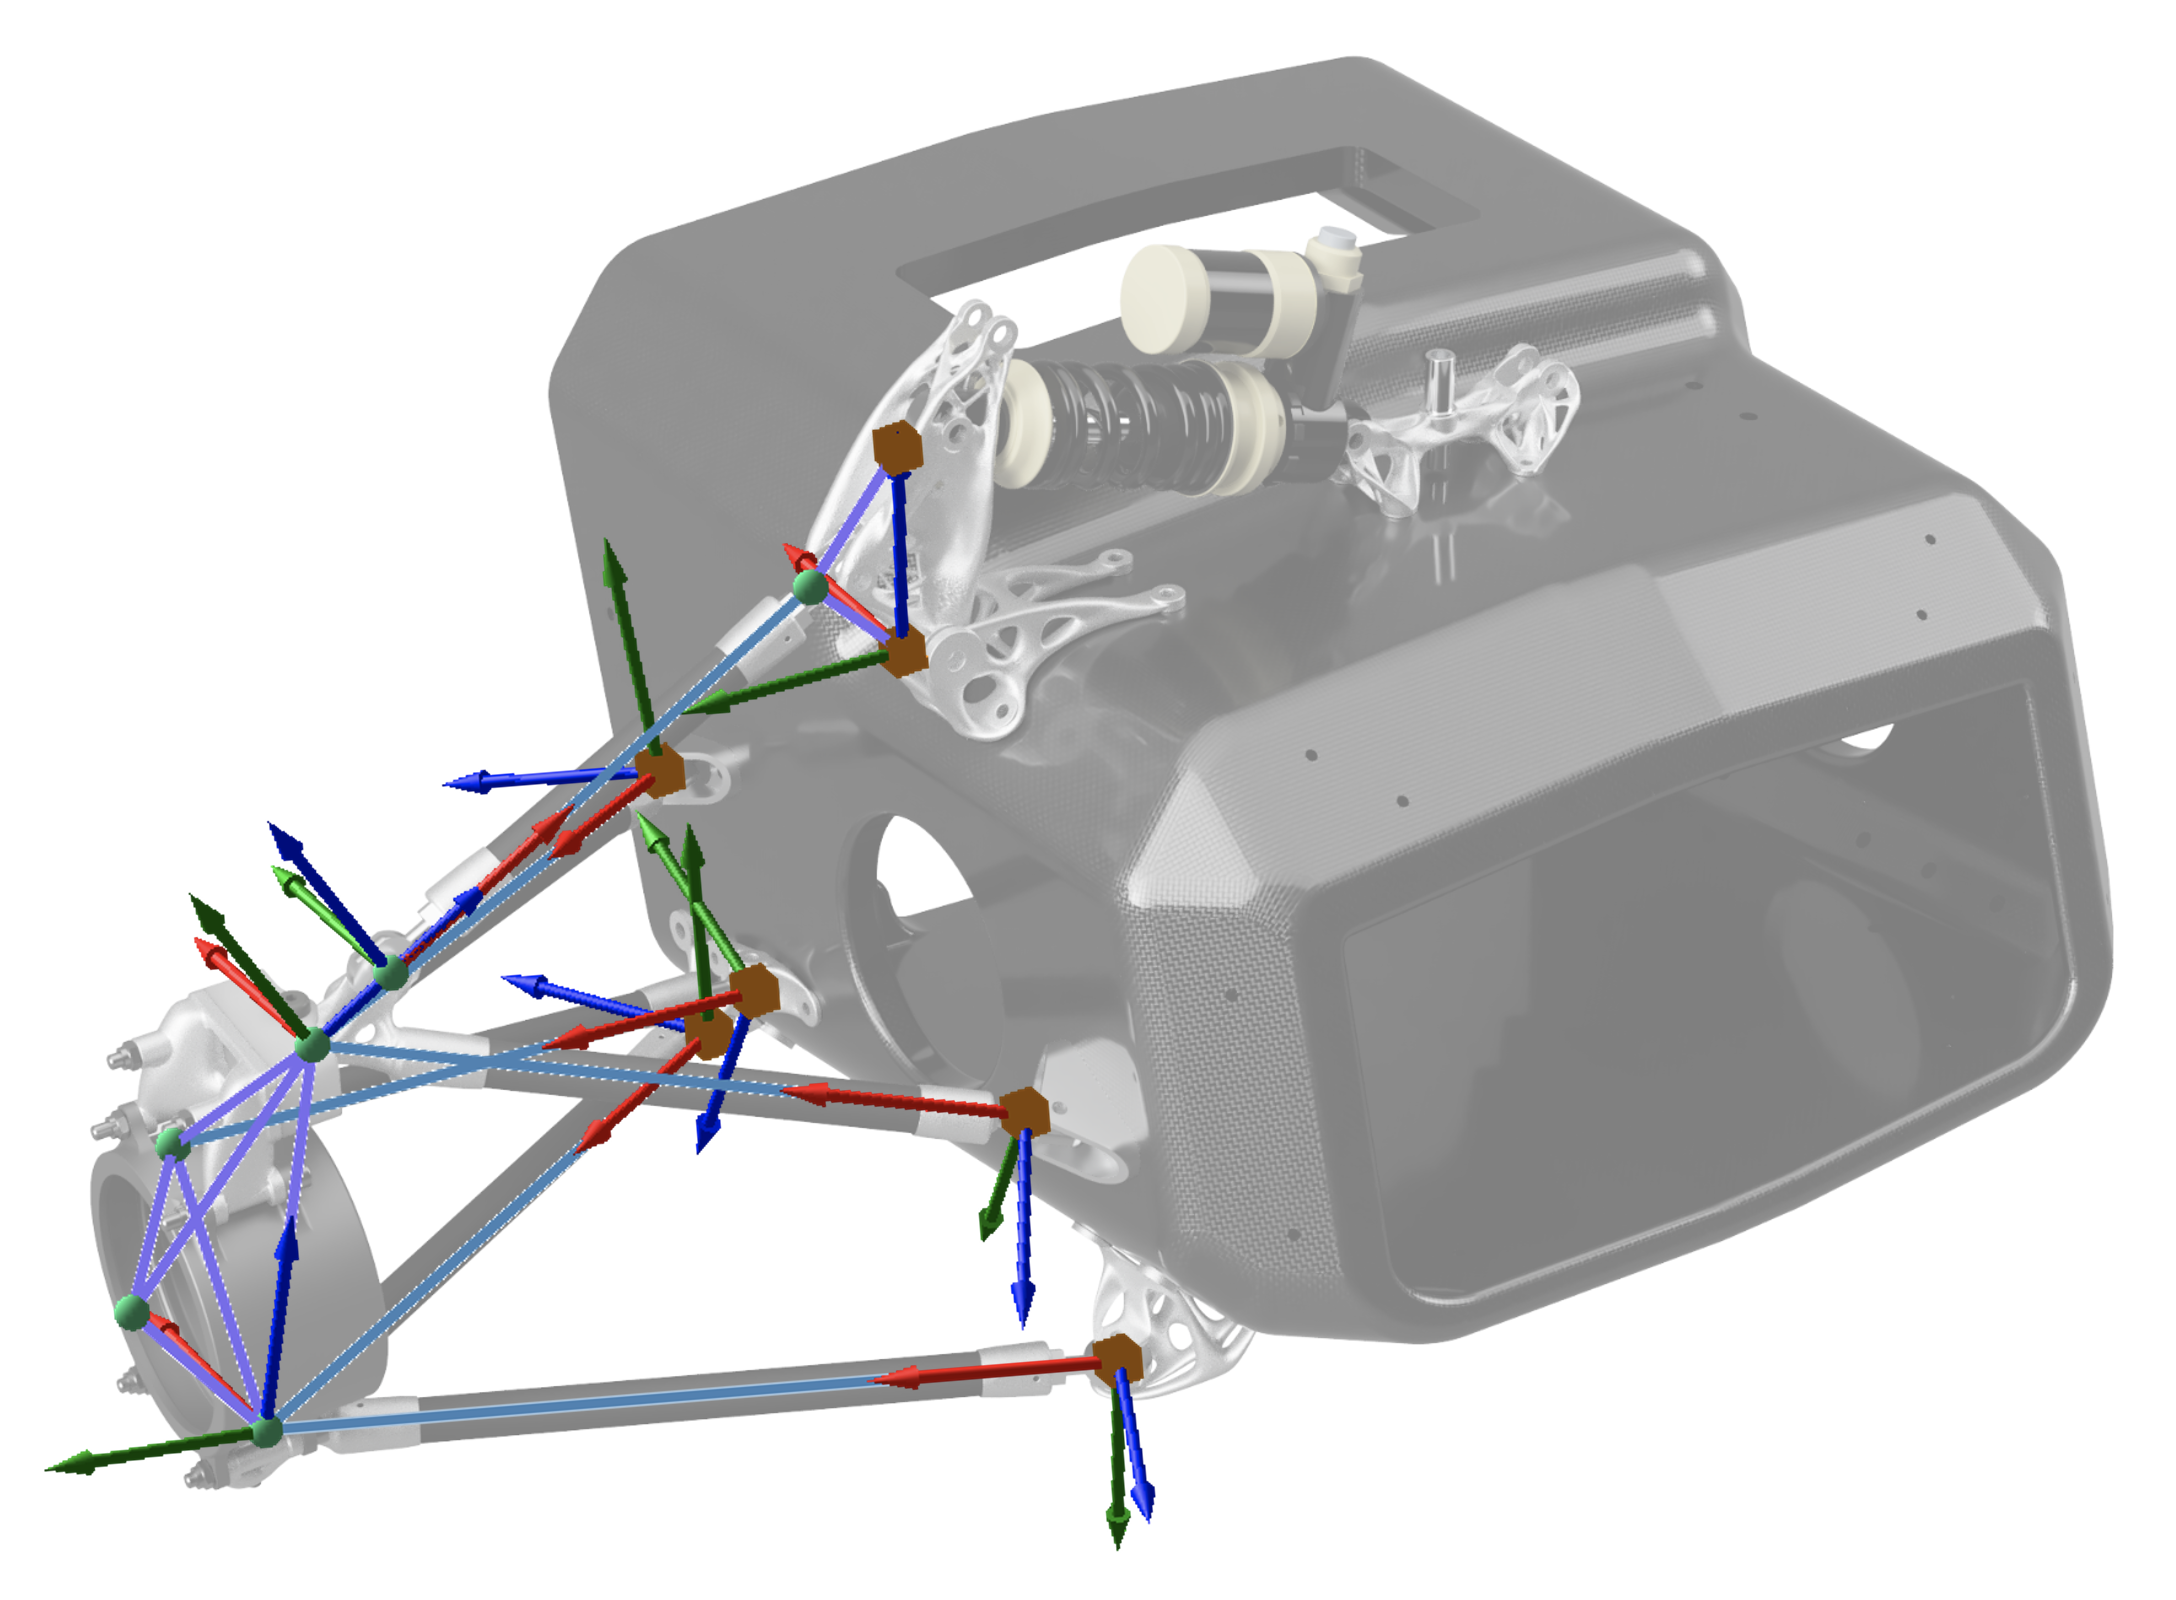
\includegraphics[width=0.4\textwidth]{figures/fade_overview.png}}
      \end{tabular}
    \end{column}
  \end{columns}
\end{frame}

\begin{frame}{Introduction and Motivation}{A Representative Example: FSAE Double Wishbone Suspension}
  \vspace{-2.0em}
  \centering{\begin{tikzpicture}[scale=0.5]
    \node at (-3,2) {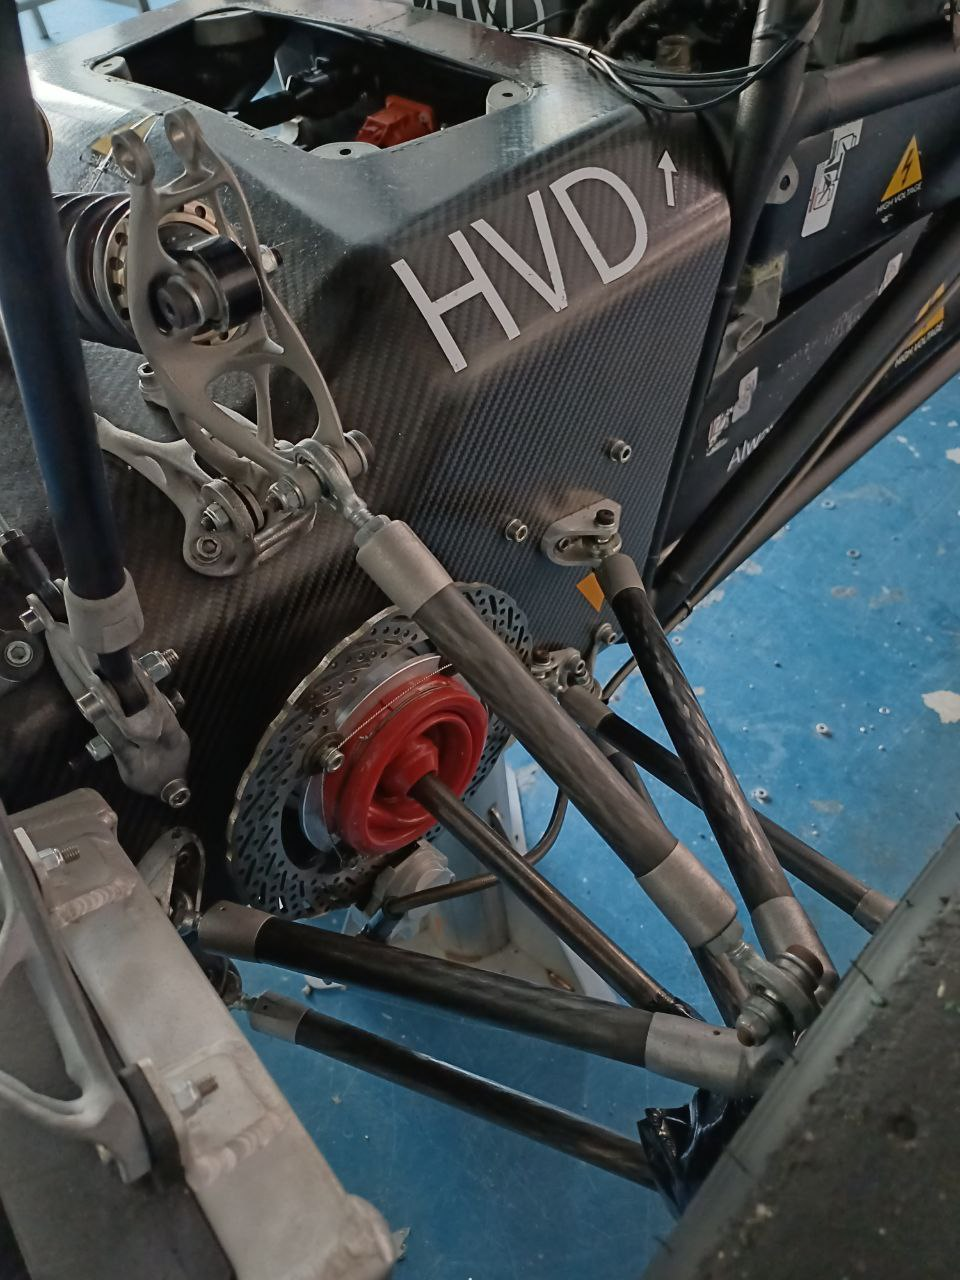
\includegraphics[width=0.125\textwidth]{figures/fsae.jpeg}};
    \node at (3,2) {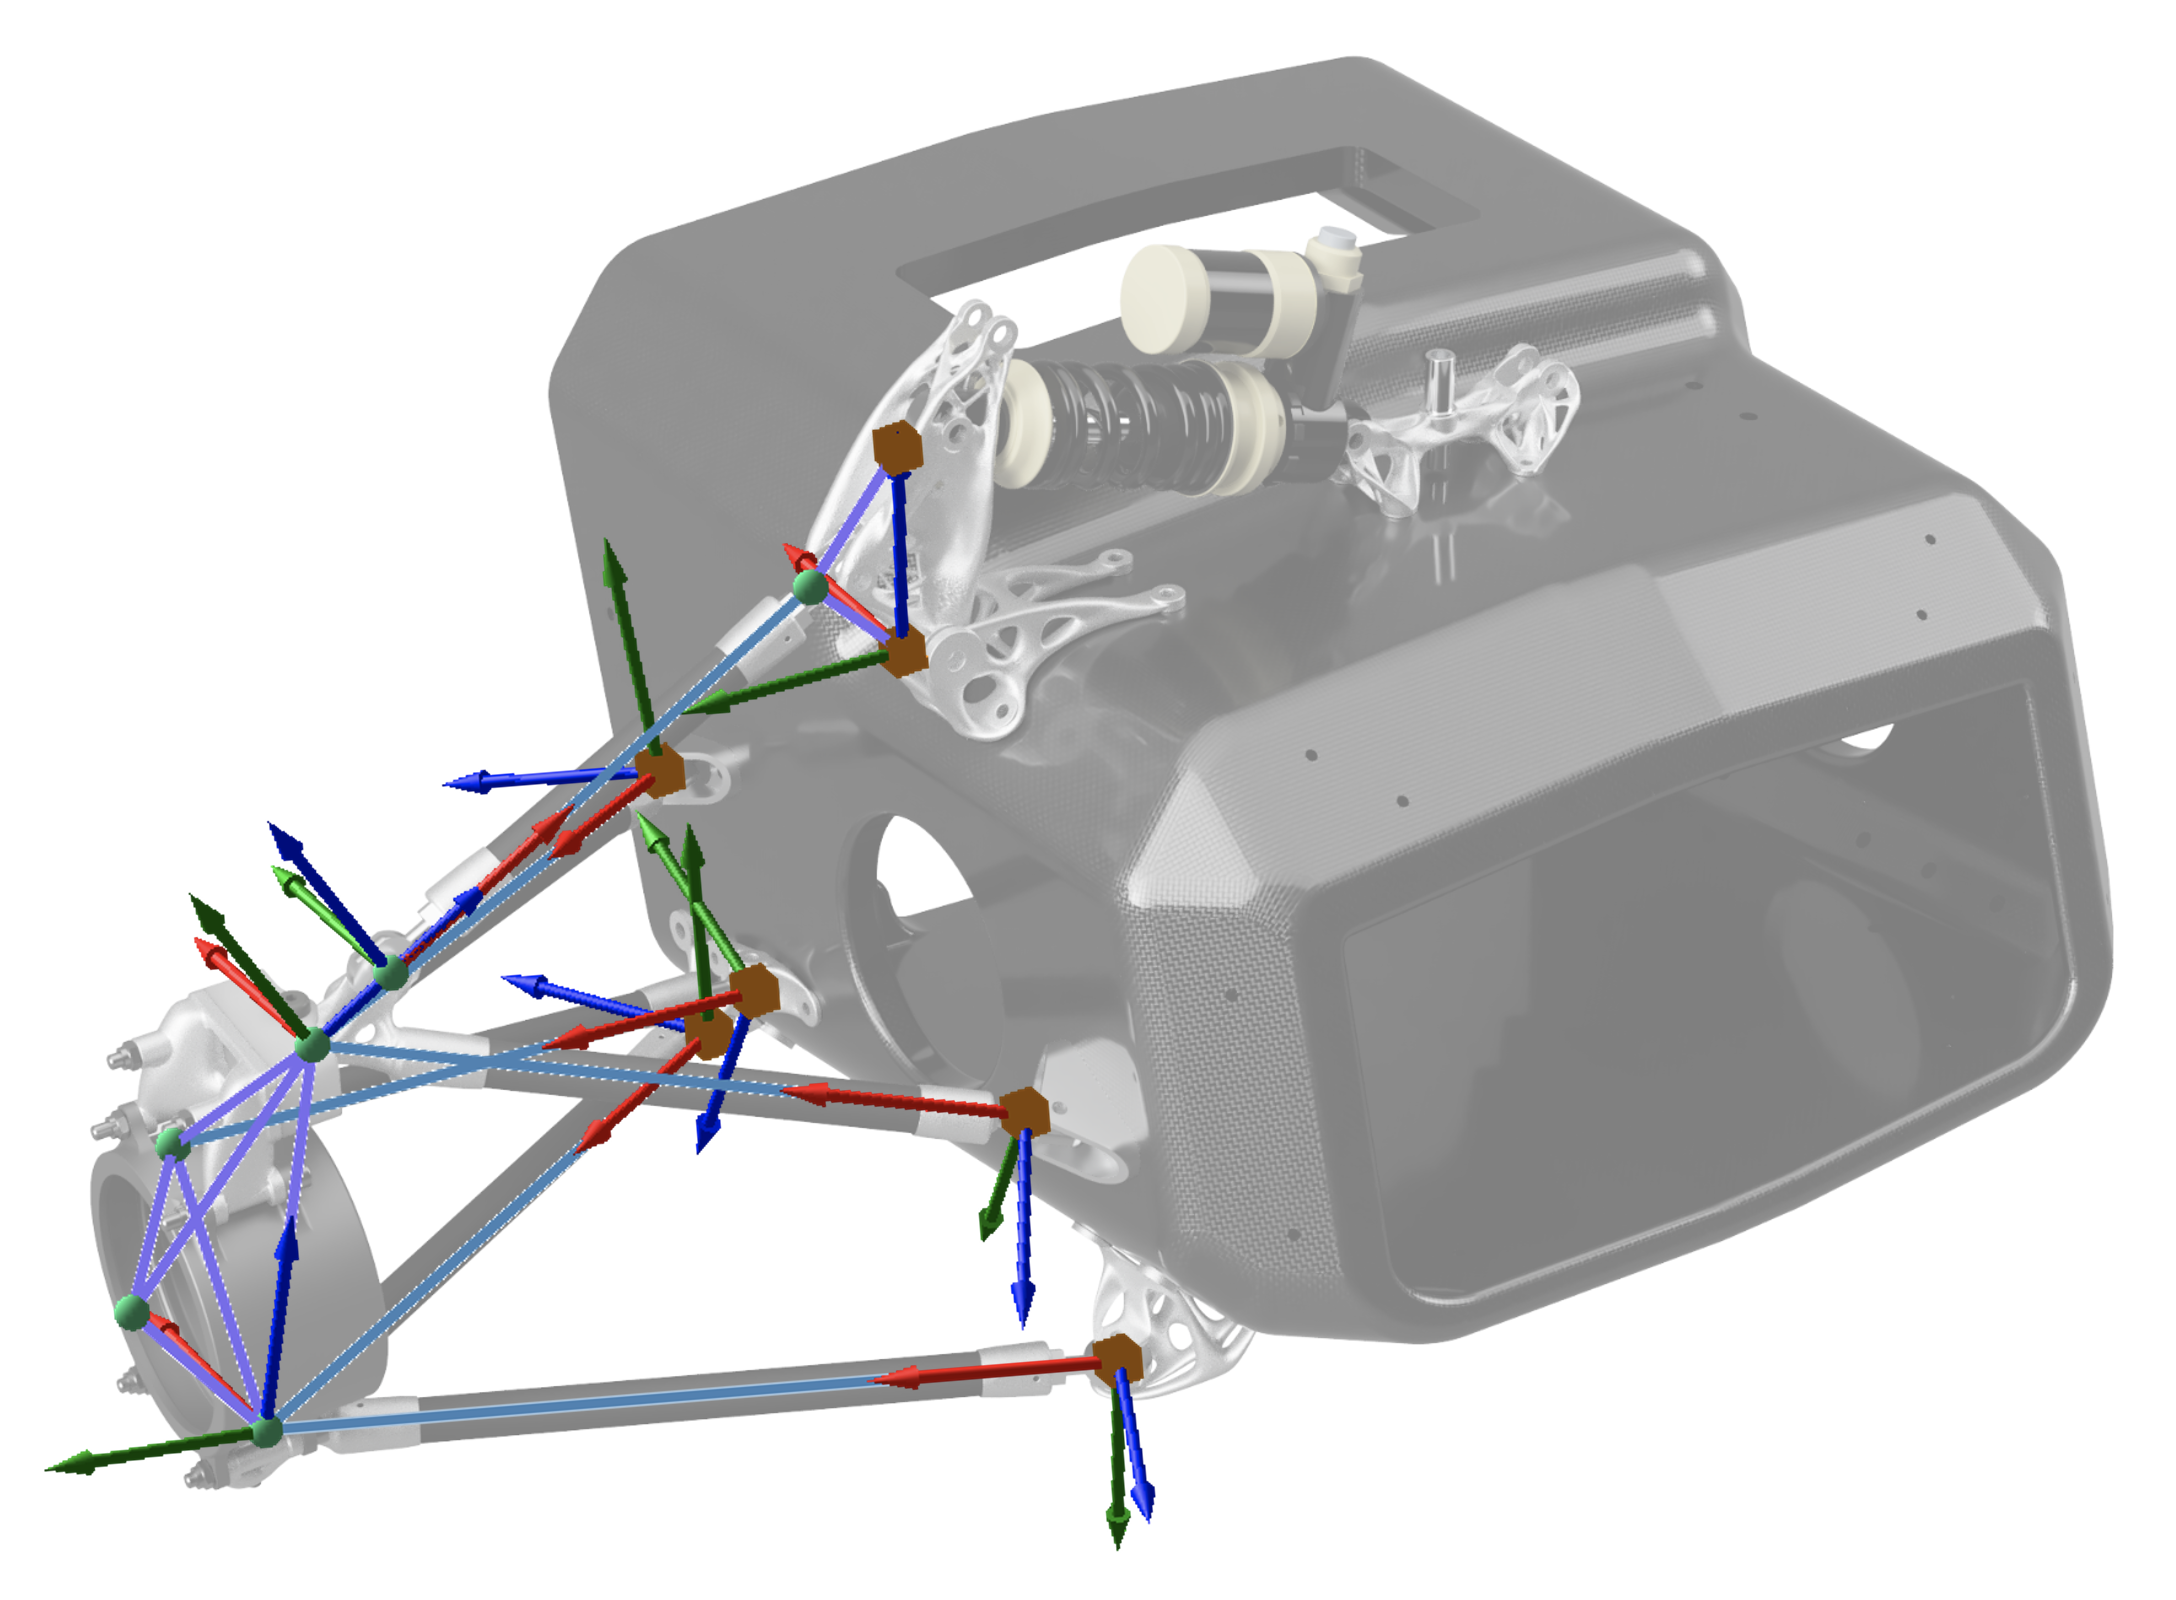
\includegraphics[width=0.25\textwidth]{figures/fade_overview.png}};
    \uncover<2->{
      \draw[fg_sl_color, thick, -stealth] (-2,-1) -- (-4.0,-3);
      \draw (-0.5\textwidth,-3.25) node[below, text width=0.5\textwidth] {
        \centering
        \hi{\large Flexibility of components} \\
        \small
        Macro-element \acs{FE} model \\[-1.5em]
        \begin{equation*}
          \begin{bmatrix}
            \mathbf{K}_{ff, 72 \times 72}(\mathbb{R}) & \mathbf{K}_{fs, 72 \times 66}(\mathbb{R}) \\
            \mathbf{K}_{sf, 66 \times 72}(\mathbb{R}) & \mathbf{K}_{ss, 66 \times 66}(\mathbb{R})
          \end{bmatrix} \begin{bmatrix}
            \mathbf{d}_{f, 72}(\mathbb{R}) \\
            \mathbf{d}_{s, 66}(\mathbb{R})
          \end{bmatrix} = \begin{bmatrix}
            \mathbf{f}_{f, 72}(\mathbb{R}) \\
            \mathbf{f}_{s, 66}(\mathbb{R})
          \end{bmatrix}
        \end{equation*}
        \vspace{-0.5em}
        \begin{equation*}
          \autorightarrow{\text{symbolic matrix}}{\text{factorization}} \quad
          \begin{aligned}
            \mathbf{d}_{f} &= \mathbf{K}_{ff}^{-1}\left(\mathbf{f}_{f} - \mathbf{K}_{fs}\mathbf{d}_{s}\right) \\
            \mathbf{f}_{s} &= \mathbf{K}_{sf}\mathbf{d}_{f} + \mathbf{K}_{ss}\mathbf{d}_{s}
          \end{aligned}
        \end{equation*}
    };}
    \uncover<3->{
      \draw[fg_sl_color, thick, -stealth] (+2,-1) -- (+4.0,-3);
      \draw (0.5\textwidth,-3.25) node[below, text width=0.5\textwidth] {
        \centering
        \hi{\large Dynamics of the system} \\
        \small
        Modified \acs{MB}-\acs{DAE} system \\[-1.5em]
        \begin{equation*}
          \left\{\!\!\!\!\begin{array}{l}
            \mathbf{y} = \mathbf{x} + \mathbf{d} \\
            \mathbf{M}(\mathbf{y}) \ddot{\mathbf{y}} + \mathbf{r}(\mathbf{x}, \dot{\mathbf{x}}, \mathbf{d}, \dot{\mathbf{d}}) = \mathbf{f}(t) \\
            \boldsymbol{\Phi}_{\mathbf{x}}(\mathbf{x})^\top \boldsymbol{\lambda} = \mathbf{K}_c(\mathbf{x}) \mathbf{d} + \mathbf{C}_c(\mathbf{x}) \dot{\mathbf{d}} + \mathbf{b}(\mathbf{x}, \dot{\mathbf{x}}, t) \\
            \boldsymbol{\Phi}(\mathbf{x}) = \mathbf{0}
          \end{array}\!\!\!\!\right.
        \end{equation*}
      };}
  \end{tikzpicture}}
\end{frame}

\subsection{Dynamic Systems Described by \acsp{ODE} and \acsp{DAE}}

\begin{frame}{Introduction and Motivation}{Dynamic Systems Described by \acsp{ODE} and \acsp{DAE}}
  \begin{itemize}
    \item Let us take a step back to generic \textbf{dynamic systems}
      \vspace{0.5em}
      \setlength{\tabcolsep}{3.5em}
      \centering{\small\begin{tabular}{cc}
          \hi{\acsp{ODE}}                                               & \hi{\acsp{DAE}} \\
          \textcolor{mycolor5!95!black}{Easy to initialize}            & \textcolor{mycolor2!95!black}{Hard to initialize} \\
          \textcolor{mycolor5!95!black}{Strong theoretical foundation} & \textcolor{mycolor3!95!black}{Complex theoretical foundation} \\
          \textcolor{mycolor5!95!black}{Efficient numerical methods}   & \textcolor{mycolor3!95!black}{Require \emph{ad hoc} numerical methods} \\
          \textcolor{mycolor2!95!black}{Some models do not fit}        & \textcolor{mycolor5!95!black}{State-of-the-art in modeling} \\
      \end{tabular}}
    \vspace{0.25em}
    \raggedright
    \item \acsp{ODE} have \textbf{well-enstablished} theoretical foundation, \acsp{DAE} do not
    \item Existing tools for \acsp{DAE} are not as \textbf{mature} and \textbf{efficient} as \acsp{ODE} tools
    \item From an engineering perspective, this is a \textbf{problem} (\textcolor{fg_sl_color}{\scalebox{0.8}{\faHourglassHalf\,\faDollarSign\,\faCarCrash\,\faSadTear}})
  \end{itemize}
  \uncover<2->{
    \centering
    \vspace{0.5em}
    Therefore, the question is \dots \\[-1.0em]
    \hic{\large How can we improve the state-of-the-art in the solution of \acsp{DAE}?}
  }
\end{frame}

% That's all Folks!
